\section{Formal Results}
\label{sec:formal-results}

%\begin{itemize}
%	\item Results that we rely on (petri nets, semilinear sets)
%	\item The base algorithm described in math (without any optimizations)
%	\item Time complexity
%	\item proof for correctness of bidirectional pruning
%	\item mathematical description of optimizations
%\end{itemize}




\subsection{The Algorithm (without Optimizations)}

Given a network system \(\mathcal S= (G, L, \mathit{REQ},  \mathit{RESP}, g_0, \delta, \mathit{req}, \mathit{resp})\) we run the following steps:  

%\begin{enumerate}
%	\item  
\medskip
	\noindent
	\textbf{Step 1: Serializability automaton.} 
	We define an NFA 
	\(
	\mathcal A_{\mathrm{ser}}(\mathcal S)=(Q,\Sigma,\delta^A,q_0,F)
	\), with
	\( Q=G,\;F=G,\;q_0=g_0,
	\)
	over an alphabet
	\(
	\Sigma=\{({\color{ForestGreen}\blacklozenge_{\mathit{req}}}/{\color{red}\blacklozenge_{\mathit{resp}}})
	\mid {\color{ForestGreen}\blacklozenge_{\mathit{req}}}\in\mathit{REQ},\;
	{\color{red}\blacklozenge_{\mathit{resp}}}\in\mathit{RESP}\}.
	\)
%	
%	\todo{old}
%	We define an NFA
%	\[
%	\mathcal A_{\mathrm{ser}}(\mathcal S)
%	= \bigl(Q,\Sigma,\delta,q_0,F\bigr),
%	\quad
%	Q = G,\quad F = G \;\;(\text{global states}),\quad
%	q_0 = g_0 \;\;(\text{initial state}),
%	\]
%	\[
%	\Sigma
%	= \Bigl\{
%	({\color{ForestGreen}\blacklozenge_{\mathit{req}}}\,/\,%
%	{\color{red}\blacklozenge_{\mathit{resp}}})
%	\;\Big|\;
%	{\color{ForestGreen}\blacklozenge_{\mathit{req}}}\in\mathit{REQ},\;
%	{\color{red}\blacklozenge_{\mathit{resp}}}\in\mathit{RESP}
%	\Bigr\}.
%	\]
%
We let each transition correspond to a request/response pair:
\(
\delta^A \subseteq Q \times \Sigma \times Q,
\quad q \xrightarrow{{\color{ForestGreen}\blacklozenge_{\mathit{req}}}/{\color{red}\blacklozenge_{\mathit{resp}}}} q'
\),
%old
%\(
%\delta \;\subseteq\; Q \times \Sigma_{	{\color{ForestGreen}\blacklozenge_{\mathit{req}}}\,/\,%
%	{\color{red}\blacklozenge_{\mathit{resp}}}} \times Q,
%\quad
%\bigl(q \xrightarrow{%
%	{\color{ForestGreen}\blacklozenge_{\mathit{req}}}\,/\,%
%	{\color{red}\blacklozenge_{\mathit{resp}}}%
%} q'\bigr),
%\)
%
%\;\Longleftrightarrow\;
%\begin{array}{l}
iff $\mathcal S$ is in global state $q$ and issues a request
$	{\color{ForestGreen}\blacklozenge_{\mathit{req}}}$, then upon some \textit{full serial execution} it eventually transitions to global state  $q'$ and returns response $	{\color{red}\blacklozenge_{\mathit{resp}}}$.
%\end{array}
%\]
%
%
%
%
%
%
%\begin{array}{l}
%	\mathcal S \text{ at global state } q
%	\;\text{issues}\;
%	{\color{ForestGreen}\blacklozenge_{\mathit{req}}},\\[0.5ex]
%	\text{after full completion of the request, it receives}\;
%	{\color{red}\blacklozenge_{\mathit{resp}}},\\[0.5ex]
%	\text{arriving at global state } q'
%\end{array}
%\]
%
%	
	Its language
	\(L(\mathcal A_{\mathrm{ser}}(\mathcal S))\subseteq\Sigma^*\) is exactly the set of serial
	request/response traces.
	Hence, by definition, it holds that applying the Parikh image gives the set of all multisets of request/response pairs obtained by serial executions:
	\(
	\mathsf{Ser}(\mathcal S)
	\;=\;
	\mathsf{Parikh}\bigl(L(\mathcal A_{\mathrm{ser}}(\mathcal S))\bigr)
	\;\subseteq\;\mathbb N^{\Sigma}.
	\)
%	Finally,
%	\(
%	q_0 = g_0
%	\quad\text{(the initial global state of the NS)}
%	\).
	
	
%	\smallskip
\begin{tcolorbox}[colback=black!5!white, colframe=black, boxrule=1pt]
	\textbf{Example.} For Listing~\ref{lst:MotivatingExample2NonSer}, the NS in Fig.~\ref{fig:code2ExampleNS} gives rise to the Serial NFA in Fig.~\ref{fig:code2ExampleNFA}.
	%
	A trace of request/response pairs is accepted by the NFA iff some serial execution of the program induces it.
	%	
Here, serial runs produce only ({\color{ForestGreen}$\blacklozenge_\text{main}$}/{\color{red}$\blacklozenge_1$}), and the only reachable global state is [\texttt{X=0}].
%	Due to the aforementioned construction, a string of request/response pairs is accepted by the NFA iff there exists a serial execution of the NS that induces it.
%
%	As the states encode the global variable values, and the edges encode request/response pairs for all serial executions, the  
%Specifically, in this case --- serial executions can only produce request/response pairs of the type ({\color{ForestGreen}$\blacklozenge_\text{main}$/{\color{red}$\blacklozenge_1$}}). Furthermore, the only global state reachable in serial executions, is [\texttt{X=0}]. 
	%
%	Intuitively, this corresponds to [\texttt{X=0}] being the initial global state, as well as the system's global state after every single packet exits the network in a serial execution.
	\end{tcolorbox}
	%
%	\begin{figure}[!htbp]
%		\centering
%		% 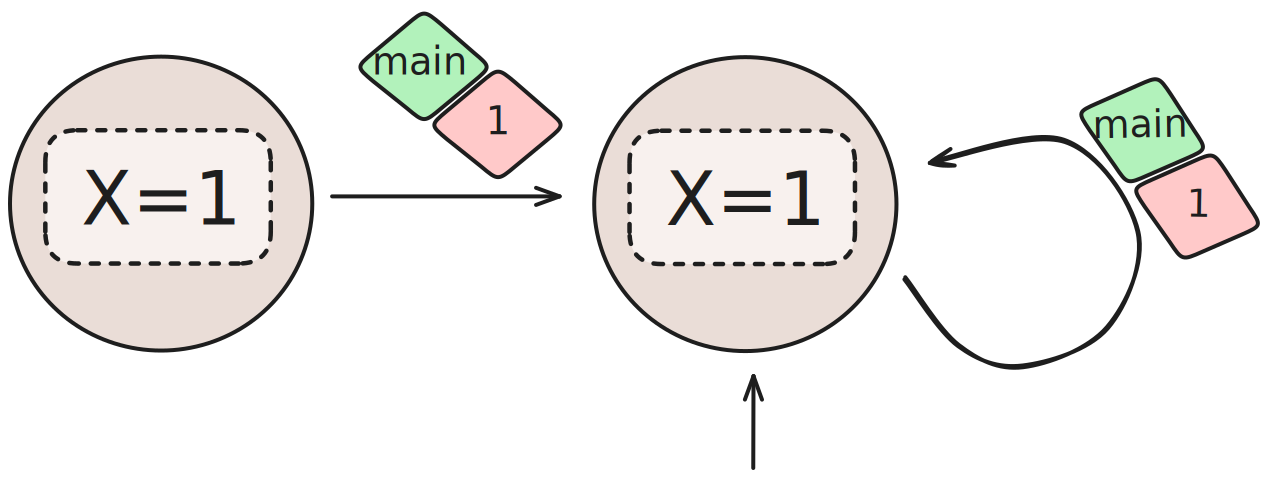
\includegraphics[width=0.48\textwidth,trim=0 0 0 0,clip]{plots/code_2_NFA_v3.pdf}
%		
%		\begin{tikzpicture}[
%			->,>=stealth,
%			thick,
%			node distance=2.5cm,
%			state/.style={
%				draw=black,
%				line width=0.8pt,
%				fill=blue!10,
%				rectangle,
%				rounded corners=1pt,
%				inner sep=2pt,
%				font=\small
%			},
%			every node/.style={font=\small}
%			]
%			% States using the same notation as section 3
%			\node[state] (X1) {\texttt{X=1}};
%			\node[state, right of=X1] (X0) {\texttt{X=0}};
%			
%			% Initial state arrow
%			\draw[->] ([yshift=-0.4cm]X0.south) -- (X0.south);
%			
%			% Transitions with proper colored notation from the paper
%			\draw[->] (X1) -- node[above] {${\color{ForestGreen}\blacklozenge_{\mathrm{main}}}/{\color{red}\blacklozenge_1}$} (X0);
%			\draw[->] (X0) edge[loop right] node[right] {${\color{ForestGreen}\blacklozenge_{\mathrm{main}}}/{\color{red}\blacklozenge_1}$} (X0);
%		\end{tikzpicture}
%		
%		\caption{Serial NFA of Listing~\ref{lst:MotivatingExample2NonSer}.}
%		\label{fig:code2ExampleNFA}
%	\end{figure}
	
	\begin{figure}[!htbp]
		\centering
		
		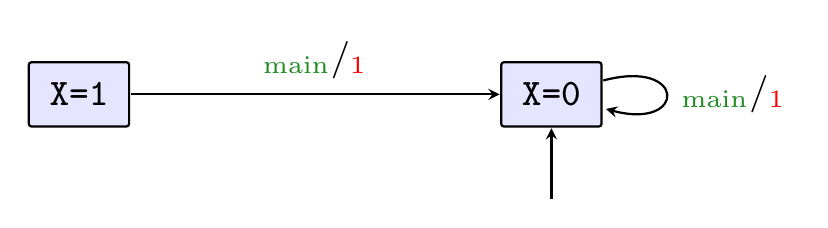
\begin{tikzpicture}[
			scale=1.5, transform shape,  % Scales the entire diagram and text
			->,>=stealth,
			thick,
			node distance=4cm, % Increased distance for better spacing
			state/.style={
				draw=black,
				line width=0.8pt,
				fill=blue!10,
				rectangle,
				rounded corners=1pt,
				inner sep=5pt, % Slightly more padding
				font=\small
			},
			every node/.style={font=\small}
			]
			% States using the same notation as section 3
			\node[state] (X1) {\texttt{X=1}};
			\node[state, right of=X1] (X0) {\texttt{X=0}};
			
			% Initial state arrow
			\draw[->] ([yshift=-0.6cm]X0.south) -- (X0.south);
			
			% Transitions with proper colored notation from the paper
			\draw[->] (X1) -- node[above] {${\color{ForestGreen}\blacklozenge_{\mathrm{main}}}/{\color{red}\blacklozenge_1}$} (X0);
			\draw[->] (X0) edge[loop right] node[right] {${\color{ForestGreen}\blacklozenge_{\mathrm{main}}}/{\color{red}\blacklozenge_1}$} (X0);
		\end{tikzpicture}
		
		\caption{Serial NFA of Listing~\ref{lst:MotivatingExample2NonSer}.}
		\label{fig:code2ExampleNFA}
	\end{figure}

	
%	\begin{wrapfigure}{r}{0.50\textwidth}  % “r” = right, width = 0.5\textwidth
%		\centering
%		% 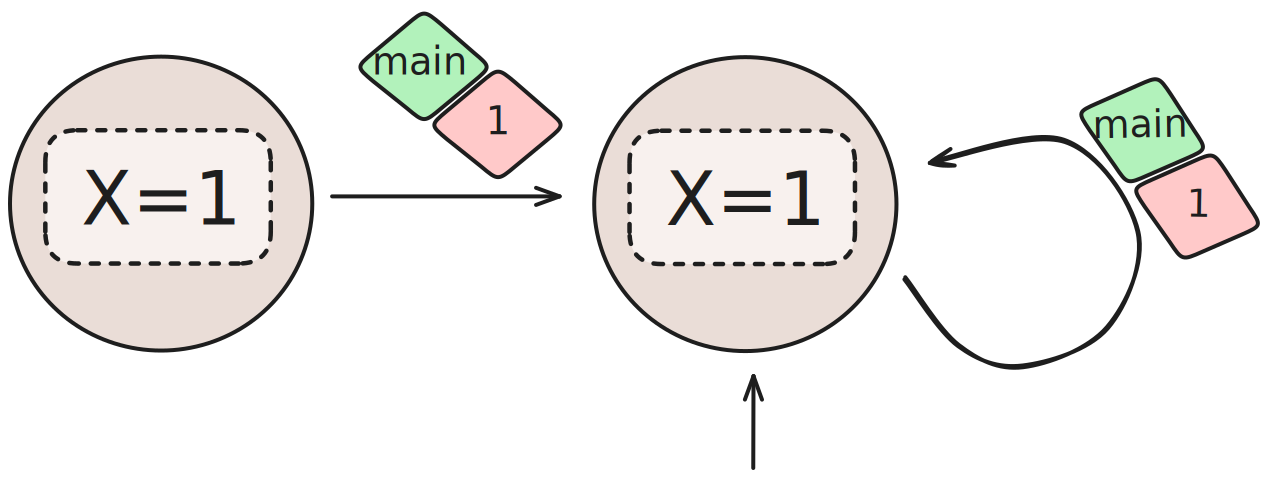
\includegraphics[width=0.48\textwidth,trim=0 0 0 0,clip]{plots/code_2_NFA_v3.pdf}
%		
%		\begin{tikzpicture}[
%			->,>=stealth,
%			thick,
%			node distance=2.5cm,
%			state/.style={
%				draw=black,
%				line width=0.8pt,
%				fill=blue!10,
%				rectangle,
%				rounded corners=1pt,
%				inner sep=2pt,
%				font=\small
%			},
%			every node/.style={font=\small}
%			]
%			% States using the same notation as section 3
%			\node[state] (X1) {\texttt{X=1}};
%			\node[state, right of=X1] (X0) {\texttt{X=0}};
%			
%			% Initial state arrow
%			\draw[->] ([yshift=-0.4cm]X0.south) -- (X0.south);
%			
%			% Transitions with proper colored notation from the paper
%			\draw[->] (X1) -- node[above] {${\color{ForestGreen}\blacklozenge_{\mathrm{main}}}/{\color{red}\blacklozenge_1}$} (X0);
%			\draw[->] (X0) edge[loop right] node[right] {${\color{ForestGreen}\blacklozenge_{\mathrm{main}}}/{\color{red}\blacklozenge_1}$} (X0);
%		\end{tikzpicture}
%		
%		\caption{Serial NFA of Listing~\ref{lst:MotivatingExample2NonSer}.}
%		\label{fig:code2ExampleNFA}
%	\end{wrapfigure}
	%
	%
	%Intuitively, this corresponds to the Listing~\ref{lst:MotivatingExample2NonSer} program updating [X:=1] as an intermediate assignment before yielding.
	
	
	
%\medskip
\noindent
%	\item 
	\textbf{Step 2: Interleaving Petri net.}
%	
Next, we translate the NS into a Petri net \(N_{\mathrm{int}}(\mathcal S)\). The \textit{non-sink places} of the PN represent either (i) global state assignments, or (ii) local states of in-flight packets. The \textit{sink places} represent request/response pairs of terminated packets.
%
We define the \textit{transitions} between states to correspond to the \(\delta\),\(req\), and \(resp\) mappings of the NS (the \(req\) transitions can fire without any input tokens in order to correspond to initializing arbitrarily many requests externally).
%
Finally, we define the initial marking \(M_0\) to be a single token in the place corresponding to the initial global state \(g_0\).
%
This construction (which is fully formalized in Appendix~\ref{appendix:NS-to-PN-formulation}) guarantees that the multiset of all reachable markings \(M\) (with \(M_0 \xrightarrow{}^{*} M\)) projected (\(\pi\)) to the sink places, corresponds to the multiset of all  (${{\color{ForestGreen}\blacklozenge_{\mathit{req}}}/{\color{red}\blacklozenge_{\mathit{resp}}}}$) pairs of the NS, as obtained by any interleaving, i.e., \(\mathsf{Int}(\mathcal S)=\{\pi(M) \mid M \in R(N_{\mathrm{int}}(\mathcal S))\}\).



\begin{tcolorbox}[colback=black!5!white, colframe=black, boxrule=1pt]
	\textbf{Example.}
%	\textit{Notation.}
In our running example, the NS gives rise to the PN in Fig.~\ref{fig:code2ExamplePN}, encoding all possible interleavings. The places \textcolor{blue}{ $P_2$} and \textcolor{blue}{$P_3$} represent the global states \textcolor{blue}{[X=1]} and \textcolor{blue}{[X=0]}, respectively, while the places $P_1$, $P_4$, $P_5$, and $P_6$ capture the local states of in-flight requests, i.e., the remaining program code coupled with the assignments to each request’s local variables. Similarly, places \textcolor{red}{$P_7$} and \textcolor{red}{$P_8$} respectively correspond to responses {\color{red}$\blacklozenge_1$} and {\color{red}$\blacklozenge_0$}. Each token either models an active request, a completed request/response pair, or --- when residing in a global-state place --- the current global state of the NS. Finally, transitions implement the network system’s mappings ($\delta/req/resp$): they either spawn a new request (e.g., transition $\textcolor{ForestGreen}{t_1}$, producing {\color{ForestGreen}$\blacklozenge_{\mathrm{main}}$} based on $req$), advance the program by one step (e.g., \(t_2,t_3,t_4,\) and \(t_5\), based on $\delta$),
or return a response (e.g., transitions $\textcolor{red}{t_6}$ and $\textcolor{red}{t_7}$, based on $resp$).
\end{tcolorbox}

%Finally, the NS gives rise to the PN in Fig.~\ref{fig:code2ExamplePN}, encoding all possible interleavings.
%%
%The places represent either the global state
%(e.g., places \textcolor{blue}{$P_2$} and \textcolor{blue}{$P_3$} correspond to the global states \textcolor{blue}{[X=1]} and \textcolor{blue}{[X=0]}), while others ($P_1,P_4,P_5,P_6$) correspond to the local state of an in-flight request, i.e., combinations of ``remaining'' programs  assignments to local variables of in-flight requests.
%%
%Furthermore, some requests correspond to responses, e.g., places \textcolor{red}{$P_7$} and \textcolor{red}{$P_8$} corresponds to {\color{red}$\blacklozenge_1$} and {\color{red}$\blacklozenge_0$}.
%%
%Each token corresponds either to a single in-flight request, a single terminated pair of request/response, or (in the case of the global-variable-encoding places), to the current global state.
%%
%Finally, transitions represent the network system's $\delta$ mapping --- encoding either a ``step'' of our program, or spawning a request ($t_1$, which  corresponds to spawning {\color{ForestGreen}$\blacklozenge_\text{main}$}), or returning a response (e.g. transitions $t_6,t_7$).
%


\begin{figure}[!htbp]
	\centering
	\includegraphics[width=1.0\textwidth]{plots/code_2_PN_with_annotation_fixed.png}
	\caption{The PN encoding interleaved executions of the program in Listing~\ref{lst:MotivatingExample2NonSer}.}
	\label{fig:code2ExamplePN}
\end{figure}



	\pagebreak
%	\medskip
	\noindent
%	\item 
	\textbf{Step 3: Non-serializable set.}  
	Let
	\(\;\mathsf{NonSer}(\mathcal S)=\mathbb N^{|\Sigma|}\setminus \mathsf{Ser}(\mathcal S)\), i.e., all multisets of (${{\color{ForestGreen}\blacklozenge_{\mathit{req}}}/{\color{red}\blacklozenge_{\mathit{resp}}}}$) pairs that \textit{cannot} be obtained via a serial execution of NS $\mathcal S$.
	
	\begin{tcolorbox}[colback=black!5!white, colframe=black, boxrule=1pt]
	\textbf{Example.}
	Regarding the aforementioned program, we automatically generate the following reachability query\footnote{If not for the equality constraints, the problem would have been considered a Petri net \textit{coverability} query, which is easier~\cite{Ra78}.} for the Petri net in Fig.~\ref{fig:code2ExamplePN}, encoding a target semilinear set by imposing the following constraints on the token distribution:
	%
	%Regarding the aforementioned program, we automatically generate the following reachability query~\footnote{If not the equality constraints, the problem would have been considered a \textit{coverability} query which is easier~\cite{Ra78}.} for the Petri net in Figure~\ref{fig:code2ExamplePN} we encode a target semilinear set with the following constraints on the token distribution:
	%
	\[
	\mathcal {F}: \quad P_1 = 0 \wedge 
	\textcolor{blue}{P_2} \ge 0 \wedge \textcolor{blue}{P_3} \ge 0  \wedge P_4 = 0
	\wedge P_5 = 0 \wedge P_6 = 0 \wedge \textcolor{red}{P_7} \ge 0 \wedge \textcolor{red}{P_8} \ge 1.
	\]
	
	This set requires no tokens on $P_1,P_4,P_5,P_6$, at least one token on $\textcolor{red}{P_8}$ (i.e., a response {\color{red}$\blacklozenge_0$}), and any number of tokens on $\textcolor{blue}{P_2},\textcolor{blue}{P_3},\textcolor{red}{P_7}$. 
	%
%	Note that \(\textcolor{red}{P_8} \ge 1\) requires at least one {\color{red}$\blacklozenge_0$}, as expected (see \Cref{sec:introduction}).
	\end{tcolorbox} 
	
	
%	\item \textbf{Reachability encoding.}  
	
%	\medskip
	\noindent
%	\item 
	\textbf{Step 4: Decision \& validation.}
	We ask whether there \textit{exists} a reachable marking \(M\) of \(N_{\mathrm{int}}(\mathcal S)\) such that \(M \models \mathcal {F}\). As \(\mathcal {F}\) encodes \(\mathsf{NonSer}(\mathcal S)\), this is equivalent to a marking \(M\) such that \(	M_0 \xrightarrow{}^{*} M\) and
	\[
	\pi(M) \in \mathsf{Int}(\mathcal S)
	\quad\wedge\quad
	\pi(M)\in \mathsf{NonSer}(\mathcal S).
	\]
	
	\begin{itemize}
		\item [\sat]: yields a counterexample interleaving \(M\) with
		\(\pi(M)\notin \mathsf{Ser}(\mathcal S)\), validated by simulation of the network system \(\mathcal S\).
%		We validate a reachable trace and embed it into the NS semantics, yielding a valid interleaving that produces request/response pairs unattainable under any serial execution.
		
		\item [\unsat]: yields an inductive invariant of
		\(N_{\mathrm{int}}(\mathcal S)\), back-translated to an NS-level proof of serializability 
%		(Appendix~\ref{appendix:ns-serializable}).
%		
%		which back-translates to an NS-level proof of
%		serializability 
%		for \(\mathcal S\)
		%
%		back-translated to a validated by synthesizing an inductive invariant over the interleaving PN, thereby proving that the corresponding semilinear set cannot be realized by any interleaving 
(see an example in Appendix~\ref{appendix:ns-serializable}).
	\end{itemize}

\begin{tcolorbox}[colback=black!5!white, colframe=black, boxrule=1pt]
	\textbf{Example.}
	In our running example, the target semilinear set \(\mathcal {F}\) is, in fact, reachable. For instance, it includes the following marking:
	
	\[
	M^* = \{\textcolor{blue}{P_3}(1),\;\textcolor{red}{P_7}(1),\;\textcolor{red}{P_8}(1)\}
	\]
	
	which is reachable by the PN in Fig.~\ref{fig:code2ExamplePN}. The full firing sequence leading to marking $M^*$ is given in Table~\ref{tab:PetriNetFiringCounterexample} .
	%
%	As the target set encodes request/response pairs that are \textit{unattainable} via serial executions, and as the PN encodes all possible interleavings, this firing sequence also corresponds as a counterexample demonstrating the program is non-serializable. 
	%
	Specifically, this reachable marking encodes the outputs $\{{\color{ForestGreen}\blacklozenge_\text{main}}/{\color{red}\blacklozenge_0},{\color{ForestGreen}\blacklozenge_\text{main}}/{\color{red}\blacklozenge_1}\}$ which, indeed, can only be induced by a non-serial execution of Listing~\ref{lst:MotivatingExample2NonSer}.
\end{tcolorbox} 



\todo{check table}
\begin{table}[!htbp]
	\centering
	\caption{The firing sequence reaching marking $M^*$ which is in our target semilinear set $\mathcal{F}$. 
		The marking $P_i(n_j)$ indicates that there are $n_j$ tokens in place $P_i$. 
		The initial marking has a single token in place \textcolor{blue}{$P_3$}, encoding $g_0$ (\textcolor{blue}{[X=0]}).}
	\label{tab:PetriNetFiringCounterexample}
	
	\small
	\begin{tabular}{c l c c c c c c}
		\toprule
		\textbf{Step} 
		& \textbf{Firing} 
		& \multicolumn{3}{c}{\textbf{Marking (after firing)}} 
		& \multicolumn{3}{c}{\textbf{Description (after firing)}} \\
		\cmidrule(lr){3-5} \cmidrule(lr){6-8}
		& & \textbf{Global} & \textbf{Local} & \textbf{Responses} 
		& \textbf{Global state} & \textbf{In-flight requests} & \textbf{Responses} \\
		\midrule
		0 & -- & {\color{blue}$P_3$(1)} & -- & -- & {\color{blue}[X=0]} & -- & -- \\
		\midrule
		1 & $\textcolor{ForestGreen}{t_1}$ & {\color{blue}$P_3$(1)} & $P_1$(1) & -- & {\color{blue}[X=0]} & {\color{ForestGreen}$\blacklozenge_\text{main}$} & -- \\
		\midrule
		2 & $\textcolor{ForestGreen}{t_1}$ & {\color{blue}$P_3$(1)} & $P_1$(2) & -- & {\color{blue}[X=0]} & \begin{tabular}[t]{@{}c@{}}{\color{ForestGreen}$\blacklozenge_\text{main}$}, \\ {\color{ForestGreen}$\blacklozenge_\text{main}$}\end{tabular} & -- \\
		\midrule
		3 & $t_3$ & {\color{blue}$P_2$(1)} & \begin{tabular}[t]{@{}c@{}}$P_1$(1),\\$P_4$(1)\end{tabular} & -- & {\color{blue}[X=1]} & \begin{tabular}[t]{@{}c@{}}{\color{black}$\blacklozenge_\text{until yield}$},\\{\color{ForestGreen}$\blacklozenge_\text{main}$}\end{tabular} & -- \\
		\midrule
		4 & $t_2$ & {\color{blue}$P_2$(1)} & $P_4$(2) & -- & {\color{blue}[X=1]} & \begin{tabular}[t]{@{}c@{}}{\color{black}$\blacklozenge_\text{until yield}$},\\{\color{black}$\blacklozenge_\text{until yield}$}\end{tabular} & -- \\
		\midrule
		5 & $t_4$ & {\color{blue}$P_3$(1)} & \begin{tabular}[t]{@{}c@{}}$P_5$(1),\\$P_4$(1)\end{tabular} & -- & {\color{blue}[X=0]} & \begin{tabular}[t]{@{}c@{}}{\color{black}$\blacklozenge_\text{after yield}$},\\{\color{black}$\blacklozenge_\text{until yield}$}\end{tabular} & -- \\
		\midrule
		6 & $\textcolor{red}{t_6}$ & {\color{blue}$P_3$(1)} & $P_4$(1) & {\color{red}$P_7$(1)} & {\color{blue}[X=0]} & {\color{black}$\blacklozenge_\text{until yield}$} & {\color{red}$\blacklozenge_1$} \\
		\midrule
		7 & $t_5$ & {\color{blue}$P_3$(1)} & $P_6$(1) & {\color{red}$P_7$(1)} & {\color{blue}[X=0]} & {\color{black}$\blacklozenge_\text{after yield}$} & {\color{red}$\blacklozenge_1$} \\
		\midrule
		8 & $\textcolor{red}{t_7}$ & {\color{blue}$P_3$(1)} & -- & \begin{tabular}[t]{@{}c@{}}{\color{red}$P_7$(1)},\\{\color{red}$P_8$(1)}\end{tabular} & {\color{blue}[X=0]} & -- & \begin{tabular}[t]{@{}c@{}}{\color{red}$\blacklozenge_0$},\\{\color{red}$\blacklozenge_1$}\end{tabular} \\
		\bottomrule
	\end{tabular}
\end{table}



%\item \textbf{Validation.}  
%
%	\begin{itemize}
%		
%		\item[\sat]: 
%		See the example in subsec.~\ref{subsec:ns-not-serializable}.
%		
%%		\item[\unsat]: 
%		
%		
%	\item \sat: we validate the reachable trace and project it to the NS semantics to represent a valid interleaving that results into request/response pairs which cannot be attained in serial executions.
%	See example in subsec.~\ref{subsec:ns-not-serializable}.
	
%	\item \unsat:
%	we generate an inductive invariant over the interleaving PN, proving that the semilinear set cannot be attained via an interleaving.
%	See example in subsec.~\ref{subsec:ns-serializable}.
%\end{itemize}

%\end{enumerate}

%\medskip
%\noindent
%\textbf{Complexity analysis.}
\subsection{Complexity Analysis}

The core algorithm reduces serializability checking to Petri net reachability with target semilinear sets. 
Since the serial executions form a regular language (step 1), their Parikh image is effectively semilinear by Parikh's theorem, with size exponential in the NFA.
The interleaving Petri net (step 2) has $O(|G| + (|\mathit{REQ}| \times |L|) + (|\mathit{REQ}| \times |\mathit{RESP}|))$ places and $O(|\mathit{REQ}|\times (1+ |\delta| + |\mathit{RESP}|))$ transitions.
The reachability query (step 3) asks whether the Petri net can reach the complement of a semilinear set, which is decidable but \texttt{Ackermann}-complete~\cite{CzWo22,Le22}.
Without optimizations, even simple examples can generate Petri nets with hundreds of places and exponentially-sized semilinear constraints, making the approach impractical.
Our optimizations (see subsec.~\ref{sec:optimizations}) \textit{drastically} reduce both the Petri net size and the semilinear set complexity, as we elaborate next.


%\guy{should we add/prove the following?}
%
%\begin{proposition}
%	Let $N_{\mathrm{int}}(\mathcal S)=(P,T,\mathsf{pre},\mathsf{post},M_0)$ be the interleaving Petri net constructed above, and let
%	\[
%	\pi\colon\mathbb N^P\to\mathbb N^{P_R}
%	\]
%	be the projection onto the request/response places $P_R$.  Then
%	\[
%	\mathsf{Int}(\mathcal S)
%	\;=\;
%	\{\;\pi(M)\;\mid\;M_0\xrightarrow{*}M\}.
%	\]
%\end{proposition}

